\begin{figure}[H]
\begin{adjustwidth}{}{-0in}
\begin{center}
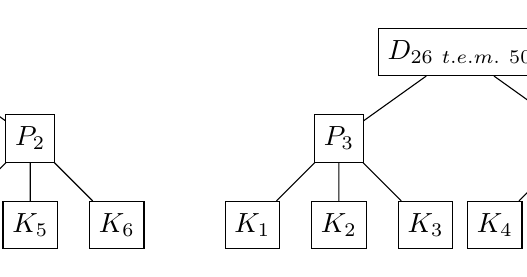
\begin{tikzpicture}[
scale=0.55,
level distance=20mm,
level 1/.style={sibling distance=56mm},
level 2/.style={sibling distance=20mm},
level 3/.style={sibling distance=12mm},
level 4/.style={sibling distance=12mm}
]

\usetikzlibrary{shapes}
\tikzstyle{c} = [draw, shape=rectangle, minimum size = 6mm]
\tikzstyle{r} = [draw, shape=rectangle,minimum width=10mm]
\tikzstyle{tr} = [draw,isosceles triangle, shape border rotate=90, anchor=north]

\hspace*{-4.5 cm}

\node[c] {$D_{1~t.e.m.~25}$}
child{node[c]{$P_{1}$}
	child{node[c]{$K_{1}$}}
	child{node[c]{$K_{2}$}}
	child{node[c]{$K_{3}$}}
	}
child{node[c]{$P_{2}$}
	child{node[c]{$K_{4}$}}
	child{node[c]{$K_{5}$}}
	child{node[c]{$K_{6}$}}
	}
;\hspace*{7 cm}
\node[c] {$D_{26~t.e.m.~50}$}
child{node[c]{$P_{3}$}
	child{node[c]{$K_{1}$}}
	child{node[c]{$K_{2}$}}
	child{node[c]{$K_{3}$}}
	}
child{node[c]{$P_{4}$}
	child{node[c]{$K_{4}$}}
	child{node[c]{$K_{5}$}}
	child{node[c]{$K_{6}$}}
	}
;
\end{tikzpicture}
\caption{D = delinquent, P = psycholoog en K = kaart. }\label{f.gen2B}
\end{center}
\end{adjustwidth}
\end{figure}
